\section{tasks::extspec Class Reference}
\label{classtasks_1_1extspec}\index{tasks::extspec@{tasks::extspec}}
Inheritance diagram for tasks::extspec::\begin{figure}[H]
\begin{center}
\leavevmode
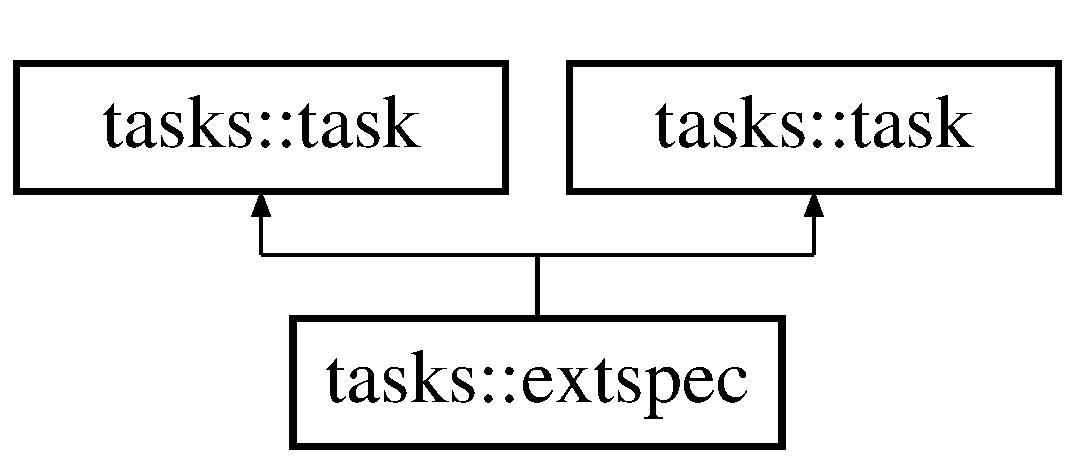
\includegraphics[height=2cm]{classtasks_1_1extspec}
\end{center}
\end{figure}
\subsection*{Public Member Functions}
\begin{CompactItemize}
\item 
def \textbf{run}\label{classtasks_1_1extspec_d8747d2d2a84687ac308a34499722371}

\item 
def \textbf{run}\label{classtasks_1_1extspec_d8747d2d2a84687ac308a34499722371}

\end{CompactItemize}
\subsection*{Static Public Attributes}
\begin{CompactItemize}
\item 
string \textbf{name} = '{\bfextspec}'\label{classtasks_1_1extspec_57fc78626df427deb4502e071327663f}

\item 
string \textbf{button\-Text} = 'Extract spectrum'\label{classtasks_1_1extspec_a9815400ea11a7ec15cca5a8bbb23da8}

\item 
string \textbf{suffix} = 'ext'\label{classtasks_1_1extspec_6c2d64ca5c93c30b4cd3c7baa2553f72}

\item 
list \textbf{prereq} = ['{\bfpreproc}']\label{classtasks_1_1extspec_030089666ca0a88ed448ed47b725760f}

\end{CompactItemize}


\subsection{Detailed Description}


\footnotesize\begin{verbatim}Extract individual orders from a two-dimensional frame using IRAF. The
   method used is the so-called 'optimal extraction'.
\end{verbatim}
\normalsize
 



The documentation for this class was generated from the following files:\begin{CompactItemize}
\item 
old/PANICtool-1.0/tasks.py\item 
old/tasks.py\end{CompactItemize}
